\documentclass[english]{../thermomemo/thermomemo}
\usepackage[utf8]{inputenc}
\usepackage{amsmath}
\usepackage{array}% improves tabular environment.
\usepackage{dcolumn}% also improves tabular environment, with decimal centring.
\usepackage{booktabs}
\usepackage{todonotes}
\presetkeys{todonotes}{inline}{}
\usepackage{subcaption,caption}
\usepackage{xspace}
\usepackage{tikz}
\usetikzlibrary{arrows}
\usetikzlibrary{snakes}
\usepackage{verbatim}
\usepackage{hyperref}
\usepackage{mhchem}
\usepackage{siunitx}
%
\usepackage{xcolor}
\hypersetup{
  colorlinks,
  linkcolor={red!50!black},
  citecolor={blue!50!black},
  urlcolor={blue!80!black}
}
%
% Kolonnetyper for array.sty:
\newcolumntype{C}{>{$}c<{$}}
\newcolumntype{L}{>{$}l<{$}}
%
\newcommand*{\unit}[1]{\ensuremath{\,\mathrm{#1}}}
\newcommand*{\uunit}[1]{\ensuremath{\mathrm{#1}}}
%\newcommand*{\od}[3][]{\frac{\mathrm{d}^{#1}#2}{\mathrm{d}{#3}^{#1}}}% ordinary derivative
\newcommand*{\od}[3][]{\frac{\dif^{#1}#2}{\dif{#3}^{#1}}}% ordinary derivative
\newcommand*{\pd}[3][]{\frac{\partial^{#1}#2}{\partial{#3}^{#1}}}% partial derivative
\newcommand*{\pdc}[3]{\frac{\partial^{2}#1}{\partial{#2}\partial{#3}}}% partial derivative
\newcommand*{\pdt}[3][]{{\partial^{#1}#2}/{\partial{#3}^{#1}}}% partial
                                % derivative for inline use.
\newcommand{\pone}[3]{\frac{\partial #1}{\partial #2}_{#3}}% partial
                                % derivative with information of
                                % constant variables
\newcommand{\ponel}[3]{\frac{\partial #1}{\partial #2}\bigg|_{#3}} % partial derivative with informatio of constant variable. A line is added.
\newcommand{\ptwo}[3]{\frac{\partial^{2} #1}{\partial #2 \partial
    #3}} % partial differential in two different variables
\newcommand{\pdn}[3]{\frac{\partial^{#1}#2}{\partial{#3}^{#1}}}% partial derivative

% Total derivative:
\newcommand*{\ttd}[2]{\frac{\mathrm{D} #1}{\mathrm{D} #2}}
\newcommand*{\td}[2]{\frac{\mathrm{d} #1}{\mathrm{d} #2}}
\newcommand*{\ddt}{\frac{\partial}{\partial t}}
\newcommand*{\ddx}{\frac{\partial}{\partial x}}
% Vectors etc:
% For Computer Modern:

\DeclareMathAlphabet{\mathsfsl}{OT1}{cmss}{m}{sl}
\renewcommand*{\vec}[1]{\boldsymbol{#1}}%
\newcommand*{\vektor}[1]{\boldsymbol{#1}}%
\newcommand*{\tensor}[1]{\mathsfsl{#1}}% 2. order tensor
\newcommand*{\matr}[1]{\tensor{#1}}% matrix
\renewcommand*{\div}{\boldsymbol{\nabla\cdot}}% divergence
\newcommand*{\grad}{\boldsymbol{\nabla}}% gradient
% fancy differential from Claudio Beccari, TUGboat:
% adjusts spacing automatically
\makeatletter
\newcommand*{\dif}{\@ifnextchar^{\DIfF}{\DIfF^{}}}
\def\DIfF^#1{\mathop{\mathrm{\mathstrut d}}\nolimits^{#1}\gobblesp@ce}
\def\gobblesp@ce{\futurelet\diffarg\opsp@ce}
\def\opsp@ce{%
  \let\DiffSpace\!%
  \ifx\diffarg(%
    \let\DiffSpace\relax
  \else
    \ifx\diffarg[%
      \let\DiffSpace\relax
    \else
      \ifx\diffarg\{%
        \let\DiffSpace\relax
      \fi\fi\fi\DiffSpace}
\makeatother
%
\newcommand*{\me}{\mathrm{e}}% e is not a variable (2.718281828...)
%\newcommand*{\mi}{\mathrm{i}}%  nor i (\sqrt{-1})
\newcommand*{\mpi}{\uppi}% nor pi (3.141592...) (works for for Lucida)
%
% lav tekst-indeks/subscript/pedex
\newcommand*{\ped}[1]{\ensuremath{_{\text{#1}}}}
\newcommand*{\ap}[1]{\ensuremath{^{\text{#1}}}}
\newcommand*{\apr}[1]{\ensuremath{^{\mathrm{#1}}}}
\newcommand*{\pedr}[1]{\ensuremath{_{\mathrm{#1}}}}
%
\newcommand*{\volfrac}{\alpha}% volume fraction
\newcommand*{\surften}{\sigma}% coeff. of surface tension
\newcommand*{\curv}{\kappa}% curvature
\newcommand*{\ls}{\phi}% level-set function
\newcommand*{\ep}{\Phi}% electric potential
\newcommand*{\perm}{\varepsilon}% electric permittivity
\newcommand*{\visc}{\mu}% molecular (dymamic) viscosity
\newcommand*{\kvisc}{\nu}% kinematic viscosity
\newcommand*{\cfl}{C}% CFL number

\newcommand*{\cons}{\vec U}
\newcommand*{\flux}{\vec F}
\newcommand*{\dens}{\rho}
\newcommand*{\svol}{\ensuremath v}
\newcommand*{\temp}{\ensuremath T}
\newcommand*{\vel}{\ensuremath u}
\newcommand*{\mom}{\dens\vel}
\newcommand*{\toten}{\ensuremath E}
\newcommand*{\inten}{\ensuremath e}
\newcommand*{\press}{\ensuremath p}
\renewcommand*{\ss}{\ensuremath a}
\newcommand*{\jac}{\matr A}
%
\newcommand*{\abs}[1]{\lvert#1\rvert}
\newcommand*{\bigabs}[1]{\bigl\lvert#1\bigr\rvert}
\newcommand*{\biggabs}[1]{\biggl\lvert#1\biggr\rvert}
\newcommand*{\norm}[1]{\lVert#1\rVert}
%
\newcommand*{\e}[1]{\times 10^{#1}}
\newcommand*{\ex}[1]{\times 10^{#1}}%shorthand -- for use e.g. in tables
\newcommand*{\exi}[1]{10^{#1}}%shorthand -- for use e.g. in tables
\newcommand*{\nondim}[1]{\ensuremath{\mathit{#1}}}% italic iflg. ISO. (???)
\newcommand*{\rey}{\nondim{Re}}
\newcommand*{\acro}[1]{\textsc{\MakeLowercase{#1}}}%acronyms etc.
\newcommand*{\ousum}[2]{\overset{#1}{\underset{#2}{\sum}}}

\newcommand{\nto}{\ensuremath{\mbox{N}_{\mbox{\scriptsize 2}}}}
\newcommand{\chfire}{\ensuremath{\mbox{CH}_{\mbox{\scriptsize 4}}}}
%\newcommand*{\checked}{\ding{51}}
\newcommand{\coto}{\ensuremath{\text{CO}_{\text{\scriptsize 2}}}}
\newcommand{\celsius}{\ensuremath{^\circ\text{C}}}
\newcommand{\clap}{Clapeyron~}
\newcommand{\subl}{\ensuremath{\text{sub}}}
\newcommand{\spec}{\text{spec}}
\newcommand{\sat}{\text{sat}}
\newcommand{\sol}{\text{sol}}
\newcommand{\liq}{\text{liq}}
\newcommand{\vap}{\text{vap}}
\newcommand{\amb}{\text{amb}}
\newcommand{\tr}{\text{tr}}
\newcommand{\crit}{\text{crit}}
\newcommand{\entr}{\ensuremath{\text{s}}}
\newcommand{\fus}{\text{fus}}
\newcommand{\flash}[1]{\ensuremath{#1\text{-flash}}}
\newcommand{\spce}[2]{\ensuremath{#1\, #2\text{ space}}}
\newcommand{\spanwagner}{\text{Span--Wagner}}
\newcommand{\triplepoint}{\text{TP triple point}}
\newcommand{\wrpt}{\text{with respect to}\xspace}
\newcommand{\excess}{\text{E}\xspace}
\newcommand{\comb}{\text{comb}\xspace}
\newcommand{\FH}{\text{FH}\xspace}
\newcommand{\SG}{\text{SG}\xspace}
\newcommand{\NC}{\text{NC}\xspace}
\newcommand{\NGr}{\text{NG}\xspace}
\newcommand{\res}{\text{R}\xspace}
\newcommand{\scomp}{\text{s}\xspace}
\newcommand{\nsc}{\text{ns}\xspace}

\title{Phase envelope modelling}
\author{Morten Hammer}

\graphicspath{{gfx/}}

\begin{document}
\frontmatter
\tableofcontents
\section{Introduction}
The intention of this memo is to describe the equations used for mapping phase envelopes in thermopack.


\section{Liquid-Vapor envelopes}

The equations:

\begin{align}
   g_i &= \ln K_i + \ln \varphi^\vap_i - \ln \varphi^\liq_i , \quad
   i=1,\dots,n \label{eq:fug_eq}\\
   g_{n+1} &= \overset{n}{\underset{i=1}{\sum}}\left(Y_i-X_i\right), \label{eq:sum_eq} \\
   g_{n+2} &= S - S_\spec \label{eq:spec_eq}.
\end{align}

Relation between overall composition and phase compositions:
\begin{align}
  \label{eq:comp1}
  \vektor{X} &= \frac{\vektor{Z}}{1-\beta+\beta \vektor{K}},\\
  \label{eq:comp2}
  \vektor{Y} &= \frac{\vektor{K}\vektor{Z}}{1-\beta+\beta \vektor{K}}.
\end{align}

Vector form of the equations:
\begin{equation}
  \label{eq:G}
  \vektor{G}\left(\vektor{W}\right) = \begin{pmatrix}
    g_1 \\
    \vdots \\
    g_{n+2}
  \end{pmatrix}
\end{equation}

Variables:
\begin{equation}
  \label{eq:W}
  \vektor{W} = \begin{pmatrix}
    \ln \vektor{K} \\
    \ln T \\
    \ln P
  \end{pmatrix}
\end{equation}
\subsection{Differentials}
The Jacobean matrix needs the following differentials:
\begin{equation}
   \pd{X_i}{\ln K_i} = -\frac{K_iZ_i\beta}{\left(1-\beta+\beta K_i\right)^2} = -\frac{K_iX_i\beta}{\left(1-\beta+\beta K_i\right)} = -\beta\frac{Y_iX_i}{Z_i}.
\end{equation}

\begin{equation}
   \pd{Y_i}{\ln K_i} = -K_i\frac{K_i Z_i\beta}{\left(1-\beta+\beta K_i\right)^2} + K_i\frac{Z_i\beta}{\left(1-\beta+\beta K_i\right)} = -\frac{\left(1-\beta\right)}{\beta}\pd{X_i}{K_i} = \left(1-\beta\right)\frac{Y_iX_i}{Z_i}.
\end{equation}

\begin{equation}
   \pd{g_i}{\ln K_j} = \delta_{ij} + \left(\left(1-\beta\right)\pd{\ln \varphi^\vap_i}{Y_j} + \beta\pd{\ln \varphi^\liq_i}{X_j}\right)\frac{X_jY_j}{Z_j}.
\end{equation}

\begin{equation}
   \pd{g_{n+1}}{\ln K_j} = \frac{X_jY_j}{Z_j}.
\end{equation}

\section{Extension to include solids}

%z = beta*Y + (1-beta-beta_\scomp)*x + beta_\scomp
%y = Kx
% sum(y) = 1
% sum(x) = 1
% phi_\scomp - phi_g*y = 0

Since $\beta$ will vary along the saturation lines, it must be included as a variable. The same applies for $\beta_\sol$. Typically one of these will be fixed to zero when mapping a three-phase line, while the other is a variable.

The equation set must be extended with the following equilibrium relation:
\begin{equation}
  \label{eq:soleq}
   g_{n+3} = \ln \varphi^\vap_\scomp + \ln Y_\scomp - \ln \varphi^\sol .
\end{equation}

Earlier it was assumed, $\beta_\vap = \beta$, and $\beta_\liq = 1-\beta$. There are three options when extending to include solids, (1) to continue to assume this within the vapor-liquid part of the mixture, or (2) to use $\beta_\liq = 1-\beta-\beta_\sol$, or (3) to introduce a new variable for $\beta_\liq$. Since we typically need to specify one of the phase fractions to be zero, only the first and the last option can be used.

For the first option, the corrected fluid composition, $Z_i^*$, becomes,
\begin{equation}
  Z_i^* = \begin{cases}
    \frac{Z_i - \beta_\sol}{1-\beta_\sol},& \text{if } i = s\\
    \frac{Z_i}{1-\beta_\sol},            & \text{otherwise}.
\end{cases}
\label{eq:z_mod}
\end{equation}

For the third option, the new mass balance for the solid component, $Z_\scomp$, becomes:
\begin{equation}
  Z_i = \begin{cases}
    \beta_\vap Y_i + \beta_\liq X_i + \beta_\sol,& \text{if } i = s\\
    \beta_\vap Y_i + \beta_\liq X_i,            & \text{otherwise}.
\end{cases}
\end{equation}
Equation \ref{eq:G} for the fluid equilibrium then changes form completely. To simplify, it is therefore suggested to use the first approach.

Substituting Equation \ref{eq:z_mod} into equations \ref{eq:comp1} we get,
\begin{equation}
  X_i = \begin{cases}
    \frac{Z_i - \beta_\sol}{\left(1-\beta_\sol\right)\left(1-\beta+\beta K_\scomp\right)},& \text{if } i = s\\
    \frac{Z_i}{\left(1-\beta_\sol\right)\left(1-\beta+\beta K_\scomp\right)},            & \text{otherwise}.
\end{cases}
 \end{equation}
To calculate $\vektor{Y}$, we still use, $Y_i=K_iX_i$.
% \begin{align}
%   X_\scomp &= \frac{Z_\scomp -\beta_\sol}{1-\beta-\beta_\sol+\beta K_\scomp},\\
%   Y_\scomp &= K_\scomp\frac{Z_\scomp -\beta_\sol}{1-\beta-\beta_\sol+\beta K_\scomp}.
% \end{align}
To calculate the real gas ($\tilde{\beta}_\vap$) and liquid ($\tilde{\beta}_\liq$) phase fractions, the mass balance for the solid component yields,
\begin{align}
  \tilde{\beta}_\vap &= \frac{Z_{is} - X_{is} +
    \beta_\sol \left( X_{is} - 1\right)}{Y_{is}-X_{is}} \\
  \tilde{\beta}_\liq &= 1 - \tilde{\beta}_\vap - \beta_\sol
\end{align}
\subsection{Additional differentials}
\begin{equation}
   \pd{X_i}{\beta} = -\frac{Z_i^*\left(K_i - 1\right)}{\left(1-\beta+\beta K_i\right)^2} = -\frac{X_i\left(Y_i - X_i\right)}{Z_i^*}.
\end{equation}

\begin{equation}
   \pd{Y_i}{\beta} = -\frac{K_i Z_i^* \left(K_i - 1\right)}{\left(1-\beta+\beta K_i\right)^2} = -\frac{Y_i\left(Y_i - X_i\right)}{Z_i^*}.
\end{equation}

\begin{equation}
  \pd{X_i}{\beta_\sol} = \begin{cases}
    \frac{X_i}{\left(1-\beta_\sol\right)}\left(1-\frac{1}{Z_i^*}\right),& \text{if } i = s\\
    \frac{X_i}{\left(1-\beta_\sol\right)},            & \text{otherwise}.
\end{cases}
 \end{equation}

\begin{equation}
   \pd{Y_i}{\beta_\sol} = K_i\pd{X_i}{\beta_\sol}.
\end{equation}

\begin{align}
   \pd{g_i}{\beta} &= -\overset{n}{\underset{j=1}{\sum}}\left(\pd{\ln \varphi^\vap_i}{Y_j}Y_j - \pd{\ln \varphi^\liq_i}{X_j}X_j\right)\frac{\left(Y_i - X_i\right)}{Z_i^*}\\
   \pd{g_{n+1}}{\beta} &= \overset{n}{\underset{i=1}{\sum}}\left(K_i-1\right)\pd{X_i}{\beta}.
\end{align}
The differential with regards to $\beta_\sol$ will have the same
shape.

\begin{equation}
   \pd{g_{n+3}}{\ln K_i} = \left(\pd{\ln
       \varphi^\vap_\scomp}{Y_i} +
     \frac{\delta_{is}}{Y_\scomp}\right) \pd{Y_i}{\ln K_j} = \left(\pd{\ln
       \varphi^\vap_\scomp}{Y_i} +
     \frac{\delta_{is}}{Y_\scomp}\right) \left(1-\beta\right)\frac{Y_iX_i}{Z_i^*}.
\end{equation}

\begin{equation}
   \pd{g_{n+3}}{\ln T} = T\left(\pd{\ln \varphi^\vap_\scomp}{T} - \pd{\ln \varphi^\sol}{T}\right).
\end{equation}

\begin{equation}
   \pd{g_{n+3}}{\ln P} = P\left(\pd{\ln \varphi^\vap_\scomp}{P} - \pd{\ln \varphi^\sol}{P}\right).
\end{equation}

\begin{equation}
   \pd{g_{n+3}}{\beta} = \overset{n}{\underset{i=1}{\sum}}\pd{\ln \varphi^\vap_\scomp}{Y_i}\pd{Y_i}{\beta} + \frac{1}{Y_\scomp}\pd{Y_\scomp}{\beta}.
\end{equation}

The differential with regards to $\beta_\sol$ will have the same shape.
\subsection{Liquid-solid or vapor-solid equilibrium}
One equilibrium and on specification equation is required,
\begin{align}
   g_{1} &= \ln \varphi^\vap_\scomp + \ln Y_\scomp - \ln \varphi^\sol,\\
   g_{2} &= S - S_\spec \label{eq:spec_eq_ls}.
\end{align}
Variables:
\begin{equation}
  \label{eq:W_ls}
  \vektor{W} = \begin{pmatrix}
    \ln T \\
    \ln P
  \end{pmatrix}
\end{equation}
One of the variables must be specified, and $\beta_\sol$ must be set. The fluid mole fractions then become,
\begin{equation}
  Y_i = \begin{cases}
    \frac{Z_\scomp - \beta_\sol}{1-\beta_\sol}, & \text{if } i = s\\
    \frac{Z_i}{1-\beta_\sol}, & \text{otherwise}.
  \end{cases}
\end{equation}

For $Y_i$ the differentials are,
\begin{equation}
  \pd{Y_i}{\beta_\sol} = \begin{cases}
    \frac{Y_i - 1}{1-\beta_\sol}, & \text{if } i = s\\
    \frac{Y_i}{1-\beta_\sol}, & \text{otherwise}.
  \end{cases}
\end{equation}
Using these the other differentials are simple.

\section{Illustrations}
Figure \ref{fig:envelope} show an example of the phase diagram of a
multicomponent mixture with approximately \SI{91}{\percent} \ce{CO2}.
\begin{figure}[ht]
  \centering
  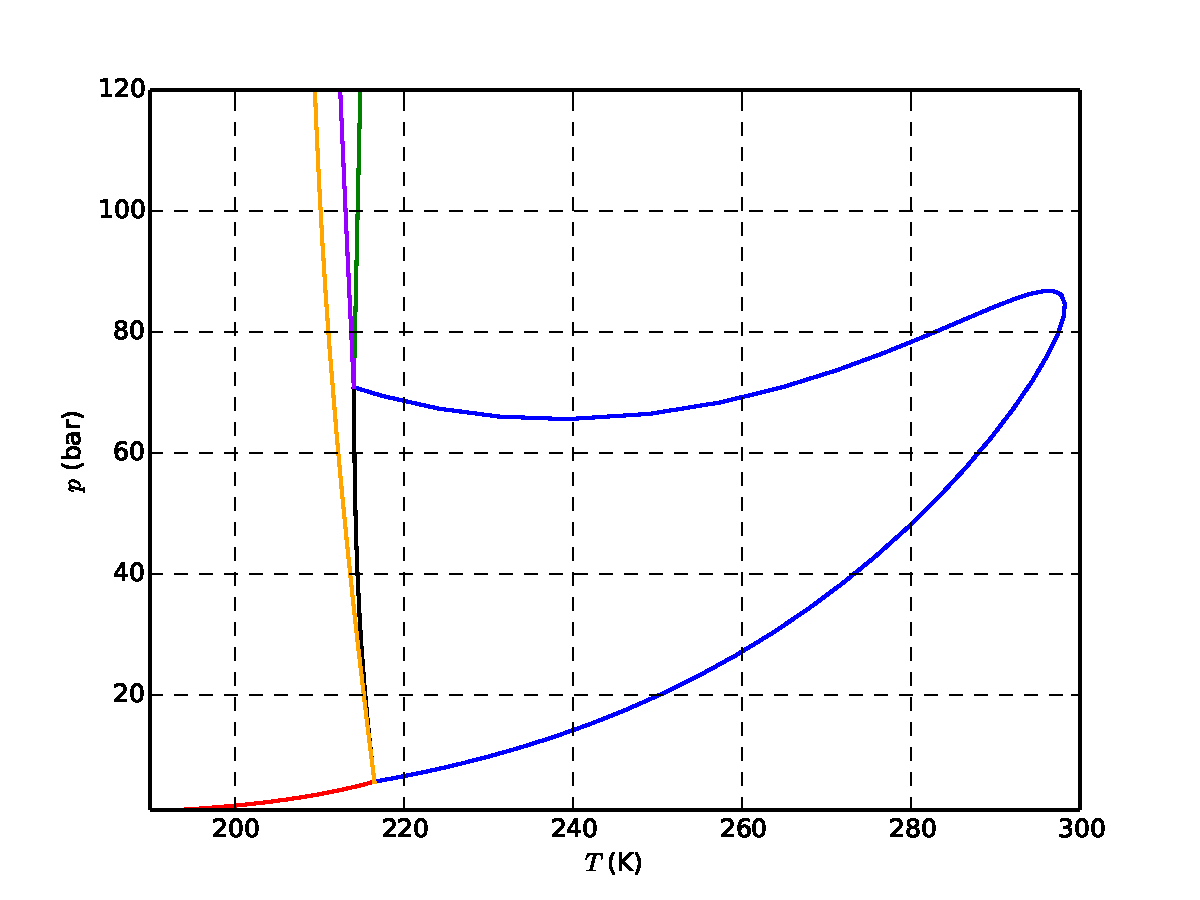
\includegraphics[width=0.6\textwidth]{envelope}
  \caption{Illustration of a multicomponent mixture
    (\ce{CO2}-\ce{H2}-\ce{N2}-\ce{O2}-\ce{CH4}) with all its phase
    areas. The blue and the black line encircle the vapor-liquid
    region. Above the red line and left of the orange line we have the
    vapor solid region. The green line is the solid appearance line in
    from the liquid phase. Right of the orange and left of the black
    and brown line there is a vapor-liquid-solid line. Between the
    purple and green line there is a liqid solid region. The mole
    fraction vector of the mixture is
    $\left[0.9094,0.0103,0.0402,0.0184,0.0217\right]$}.
  \label{fig:envelope}
\end{figure}

\section{Two-component system}
For a two-component system there is no three phase area, only a three
phase line. This means, that at the same temperature and pressure,
several equilibrium states can be found. The state differ only in
different solid fraction and different fluid phase fractions. That is;
while dry-ice freeze, the phase compositions are constant. The
chemical potential of the component freezing then remain constant, as
seen from Equation \ref{eq:soleq}.

This is illustrated in Figure \ref{fig:envelope2}. Figure
\ref{fig:envelope2} show the phase diagram of a mixture containing
\SI{87.5}{\percent} \ce{CO2} and \SI{12.5}{\percent} \ce{N2}.

\begin{figure}[ht]
  \centering
  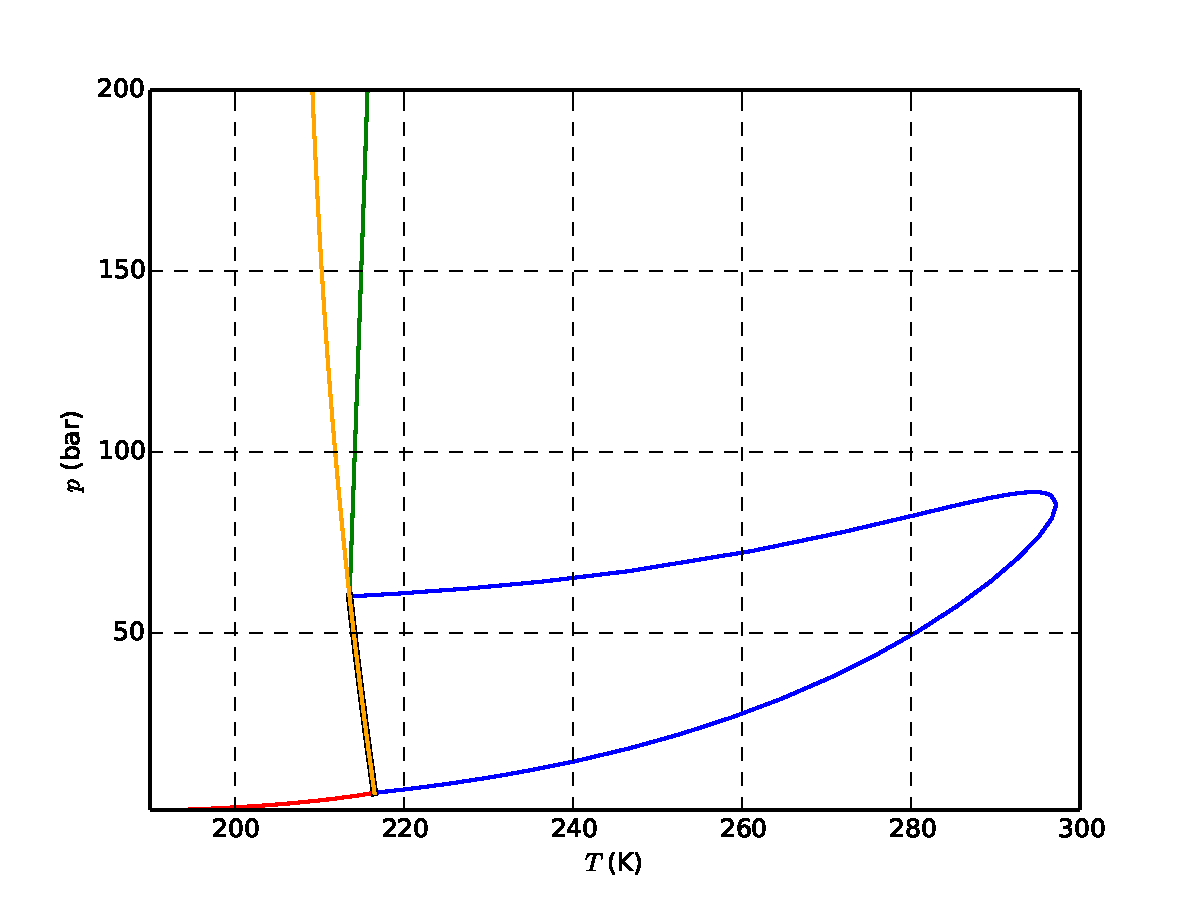
\includegraphics[width=0.6\textwidth]{envelope2}
  \caption{Illustration of a binary mixture (\ce{CO2}-\ce{N2}) with all
    its phase areas. The blue and the black line encircle the
    vapor-liquid region. Above the red line and left of the orange
    line we have the vapor solid region. The green line is the solid
    appearance line in from the liquid phase. It is seen that there is
    no three phase area, only a line, as the orange and black line
    coincide. The mole fraction vector of the mixture is
    $\left[0.875,0.125\right]$}.
  \label{fig:envelope2}
\end{figure}

The Gibbs' phase rule, state that the degree of freedom ($F$) is given
as number of components ($C$) and number of phases ($P$),
\begin{equation}
  F = C - P + 2.
\end{equation}
For three phases and two components, the degree of freedom
become 1. That is; the it is not possible to change the temperature
independently of the pressure, giving a three-phase line in
temperature-pressure space.

Applying the same rule to pure \ce{CO2}, no degree of freedom is seen
for the three-phase region, giving a triple point in
temperature-pressure space.

% \clearpage
% \bibliographystyle{plain}
% \bibliography{../thermopack}

\end{document}
